\section{Implementation}
\label{sec:implementation}



This section describes the architecture and implementation of \projecttitle. We implemented \projecttitle as a dynamically linkable shared library for the GNU/Linux OS that can be loaded and linked  at runtime for {\tt POSIX} threads (replacing the \pthreads library). The application executables can simply link the library (without any recompilation) either using {\tt LD\_PRELOAD} or the {\tt -rdynamic} flag, specifying the path of the \projecttitle library.  The \projecttitle library exports the CPG as an extended interface in the {\tt perf} utility for supporting data provenance.   The architecture of \projecttitle (shown in Figure~\ref{fig:basicSystem}) consists of two main components: threading library and OS support for \intelpt. We next describe these two components in detail.



\begin{figure}[t]

\centering
      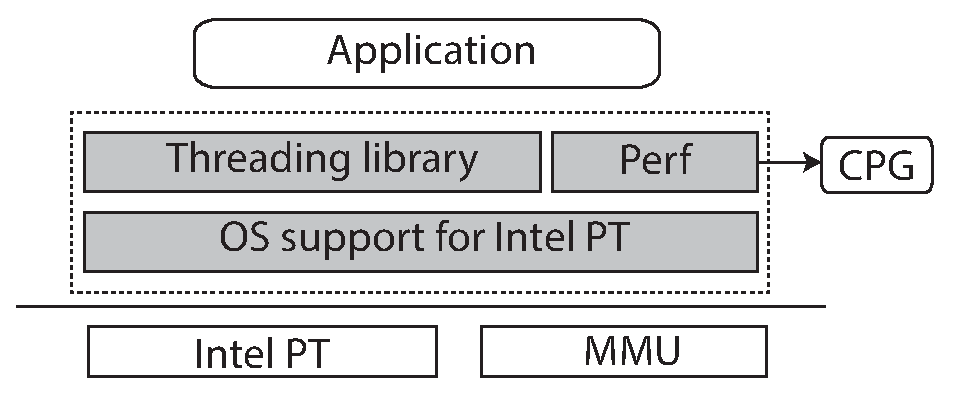
\includegraphics[scale=.4]{figure/System-basic-architecture}
  \caption{\projecttitle architecture. (System components are shown in grey boxes.)}
   
  \label{fig:basicSystem}

\end{figure}



\subsection{Threading Library}
The threading library derives the data and schedule dependencies. The architecture of the threading library is shown in Figure~\ref{fig:lib-architecture}. 

 
\myparagraph{Memory protection} A central challenge of the implementation of the algorithm is keeping track of the data dependencies for shared-memory accesses by all possible interleaving threads. Since monitoring every load and store to each memory word would be too costly, we instead rely on the OS's (hardware-assisted) page fault mechanism to keep track of reads and writes at the granularity of memory pages.

To derive the read and write sets during sub-computation execution,  \projecttitle~uses standard memory protection  mechanism and signal handlers. In particular, \projecttitle protects the address space using {\tt mprotect(PROT\_NONE)} at the beginning of each sub-computation. This forces a trap (and the corresponding OS signal) the first time a page is read or written to in a given sub-computation. The respective signal handler, which is implemented by the \projecttitle library, records the information about the access, and also resets the protection bits so that subsequent accesses to the same page by the same thread in the same sub-computation can proceed without generating a trap, and therefore avoid a
latency penalty.  

\begin{figure}[t]

\centering
      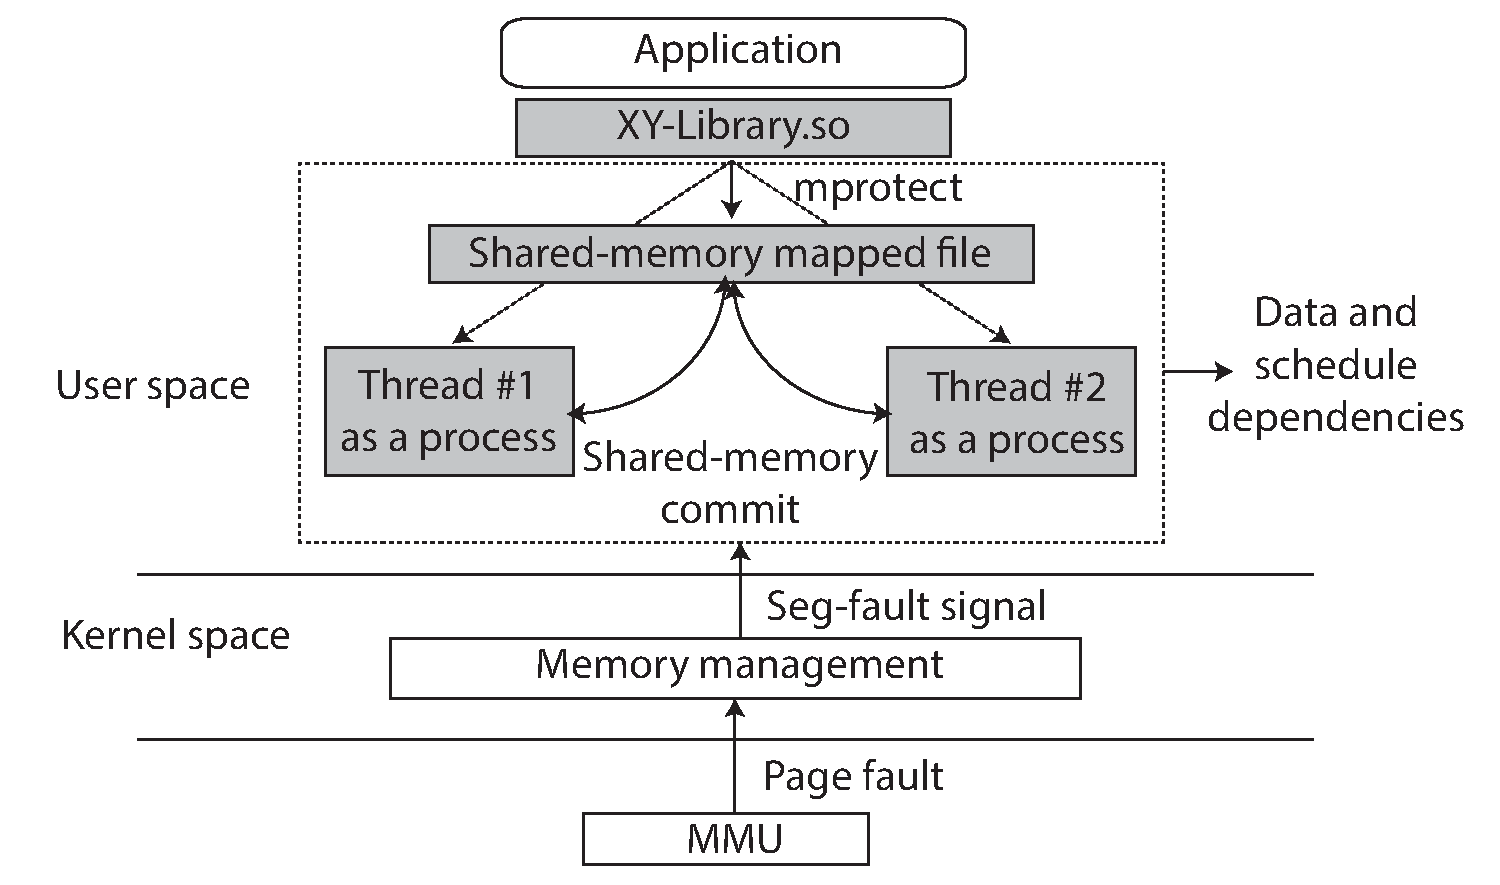
\includegraphics[scale=.3]{figure/Library-architecture}
  \caption{Threading library}
   
  \label{fig:lib-architecture}

\end{figure}

However, a naive page protection mechanism raises an important problem because all threads in a process share the same virtual memory
structures (namely the TLB and page table entries with the respective protection bits). This makes it difficult to keep track of which
threads are responsible for which memory accesses or to enforce different protections for different threads. Otherwise, we need to re-protect the page after serving every load and store instruction causing a large number of page faults.
%(E.g., an access to a given memory location may or may not be the first access in a sub-computation depending on which thread is performing the access.) 
To address this problem, \projecttitle implements threads as separate
processes (an idea originally proposed by Grace~\cite{grace-oopsla-2009}).

\myparagraph{Threads as processes} \projecttitle  implements threads as separate processes thus allowing each thread has its own private address space and control over the virtual
memory structures.   This gives us the ability to manipulate the page protection of threads individually while providing a simple way to implement the release consistency memory
model. In particular, \projecttitle uses the {\tt clone} system call to fork off a new process on {\tt pthread\_create()}. The process that implements the newly created thread (i.e., the child process) already
shares parts of the execution context with the parent process (which implements the calling thread) such as file descriptors and signal handlers. 


But this raises a new problem, which is that, unlike threads, processes do not share their address spaces. We address this by taking advantage of the RC memory model we defined for \projecttitle, where threads share the updates only at synchronization points.  

\myparagraph{Shared memory commit} To implement the RC memory model, we use shared memory commit of  Dthreads~\cite{dthreads-sosp-2011} (originally proposed in distributed shared memory architectures such as TreadMarks~\cite{treadmark})% and Munin~\cite{munin}) 
that allows threads to communicate at well-defined synchronization points.
Our shared memory commit is implemented using memory mapped files. In
particular, the virtual address ranges for the shared portions (globals and heap) of
the address space are mapped to memory mapped files, which are managed by the
\projecttitle library. These address ranges correspond to the heap and
the static (i.e., globals) regions.  During thread creation,
\projecttitle marks these address ranges as a private copy-on-write
mapping (using {\tt MAP\_PRIVATE} in {\tt mmap()}). The effect of this
is that whenever the child thread tries to write to a memory location,
the OS makes a thread-private copy of the memory page containing the
modification.  At synchronization points, the thread computes a {\em diff}
for each dirty page by performing a byte-level comparison between the
dirty page and the shared page. The deltas are then atomically
copied to the shared memory page; if there are overlapping writes
to the same memory location we resolve them using a last-writer wins policy.


\myparagraph{Input} In addition to providing wrappers for {\tt pthreads} and {\tt malloc} related API calls, we also implemented shim layer for a number of {\tt glibc} library calls for reading the input. For instance, we provide wrappers for {\tt mmap} to record the data-flow from the input. In particular, the threading library differentiates between the {\tt mmap} calls made by the library itself and the target application. This allows us to record the mapping of the input file in the input address space. And, as described before, the library uses {\tt mprotect()} to derive the data flow from the input. 


\subsection{OS Support for \intelpt}

To obtain the control flow dependencies, we use the new Intel ISA extensions, called Processor Trace (PT), recently released as part of the Broadwell (also in Skylake) microarchitecture. In Linux this processor feature is exposed to the user-space as a Performance Measuring Unit (PMU) in the {\tt perf} event interface. We make use of the \intelpt PMU to derive the control flow dependencies. Figure~\ref{fig:pt-OS-support} shows the architecture for the OS support for \intelpt.

 
\begin{figure}[t]

\centering
      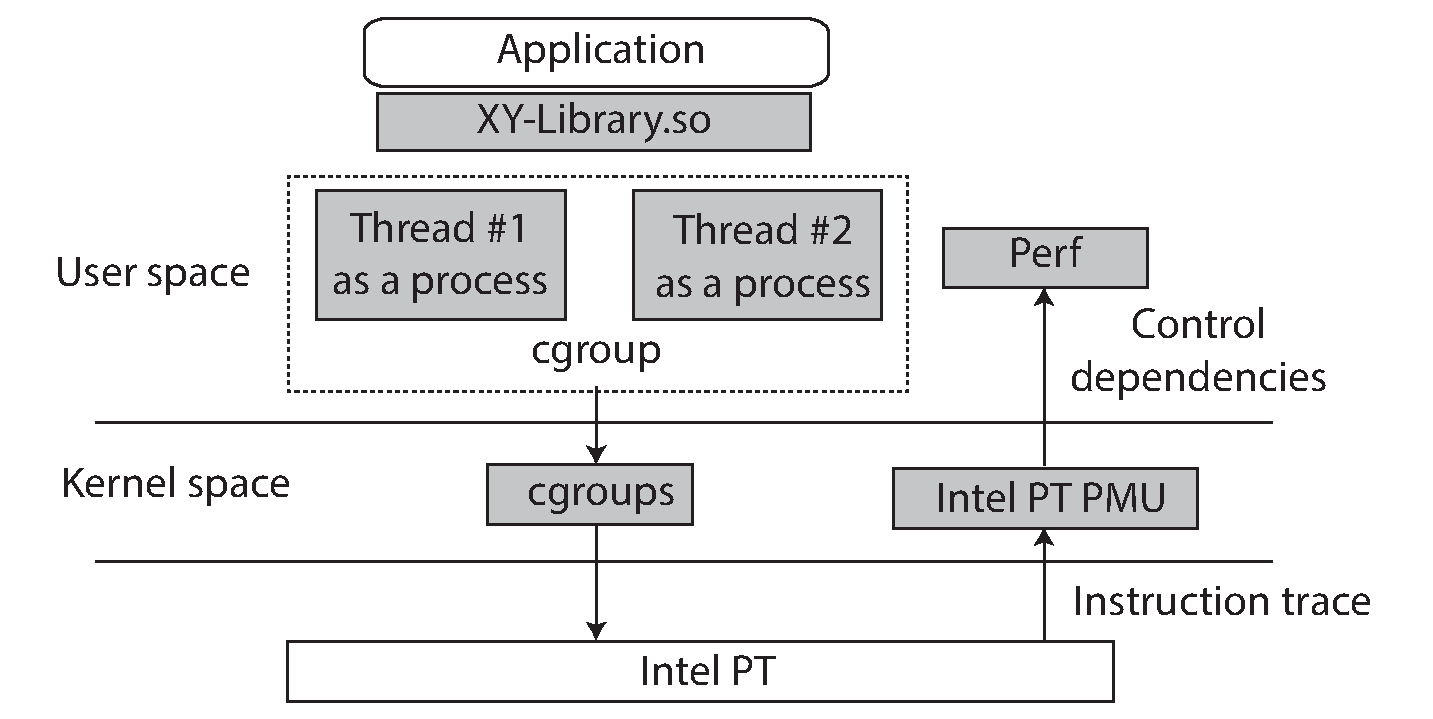
\includegraphics[scale=.35]{figure/PT-os}
  \caption{\projecttitle OS support.}
   
  \label{fig:pt-OS-support}

\end{figure}


In particular, the {\tt perf} interface on Linux consists of a syscall, which gives back a file
descriptor. Events are accessed by obtaining buffers via {\tt mmap(2)} and can be
further controlled via {\tt ioctl()} syscall on the given file descriptor. Along with
interface the user-space {\tt perf} allows to dump and filter from these
buffers. In our case, this filtering is done by using Linux control
groups (also known as {\tt cgroups}). {\tt cgroups} is a kernel feature to apply constraint
like resource usage to a group of processes. It has the property, that by
default every child process belongs to the same process as its parent. Also for
{\tt perf\_events} such a {\tt cgroup} exists.

We create such a {\tt cgroup} exclusively for the application using \projecttitle. This is done because
our threading library causes applications using threads to create multiple
processes instead, whose process ids are not known it advance.

The subcommand {\tt perf record} is then used to dump the trace produced by \intelpt.
\intelpt generates a stream of TNT packets, which denotes the
condional branches taken and TIP packets for indirect branches and function
returns. The data is referenced as a sample event in the {\tt perf} event list and
stored in a ring buffer called \emph{AUX area}. If perf tool cannot
keep up with processor trace it is possible (for example an interrupt occurs),
there will be gaps in the trace. PSB packets allow to resynchronize over these
gaps. (We also provide a snapshot facility for long running programs described in $\S$~\ref{sec:snapshot}.)


After execution the result can be further processed by using a set of tools
for example {\tt perf script}. The branch information is still in a compressed
form and needs to be decoded. The {\tt perf} utility has a decoder integrated to achieve this.
To map the trace onto binaries, it needs access to executables and linked
libraries of the application. During the execution mmap events are tracked to
know to the location of each loadable.




Along with \intelpt, page fault events generated by the kernel will be included
additionally to the trace packets. Because our threading library uses {\tt mprotect}
syscall to monitor access of heap and global memory space, whenever the
application access this memory, the MMU will generate page fault. These
page fault also includes the location, where in code memory was accessed.





%To instrument an application we use an execution wrapper. This wrapper instructs
%the runtime linker to load our library tthread by setting \emph{LD\_PRELOAD}. It
%also prepares a file, which is later on used by tthread to log the thread
%schedule and data dependence graph during execution. To obtain control flow,
%we use an new Intel ISA Extension, called Processor Trace (PT).
%In Linux this processor feature is exposed to userland as a Perfomance Measuring
%Unit (PMU) in the perf event interface.
%
%The Perf interface on Linux consists of a syscall, which gives back a file
%descriptor. Events are accessed by obtaining buffers via mmap(2) and can be
%further controlled via ioctl syscalls on the given file descriptor. Along with
%interface the userspace \emph{perf} allows to dump and filter from these
%buffers. In the case of Inspector filtering is done by using Linux control
%groups (Also known as Cgroups). Cgroups are a kernel feature to apply constraint
%like resource usage to a group of processes. It has the property, that by
%default every child process belongs to the same process as its parent. Also for
%\emph{perf\_events} such a cgroup exists. The execution wrapper will create such
%a croup exclusivly for the application under test. This is done because
%\emph{tthread} will cause applications using threads to create multiple
%processes instead, which process ids are not known it advance.
%
%The subcommand \emph{perf record} is then used to dump the trace produced by PT.
%Intel PT generates their for a stream of TNT packets, which denotes the
%condional branches taken and TIP packets for indirect branches and function
%returns. The data is referenced as a sample event in the perf event list and
%stored in a ring buffer called \emph{AUX area}. If perf tool cannot
%keep up with processor trace it is possible (for example an interrupt occurs),
%theire will be gaps in the trace. PSB packets allow to resynchronize over these
%gapps.
%
%
%
%
\begin{figure}[t]

\centering
      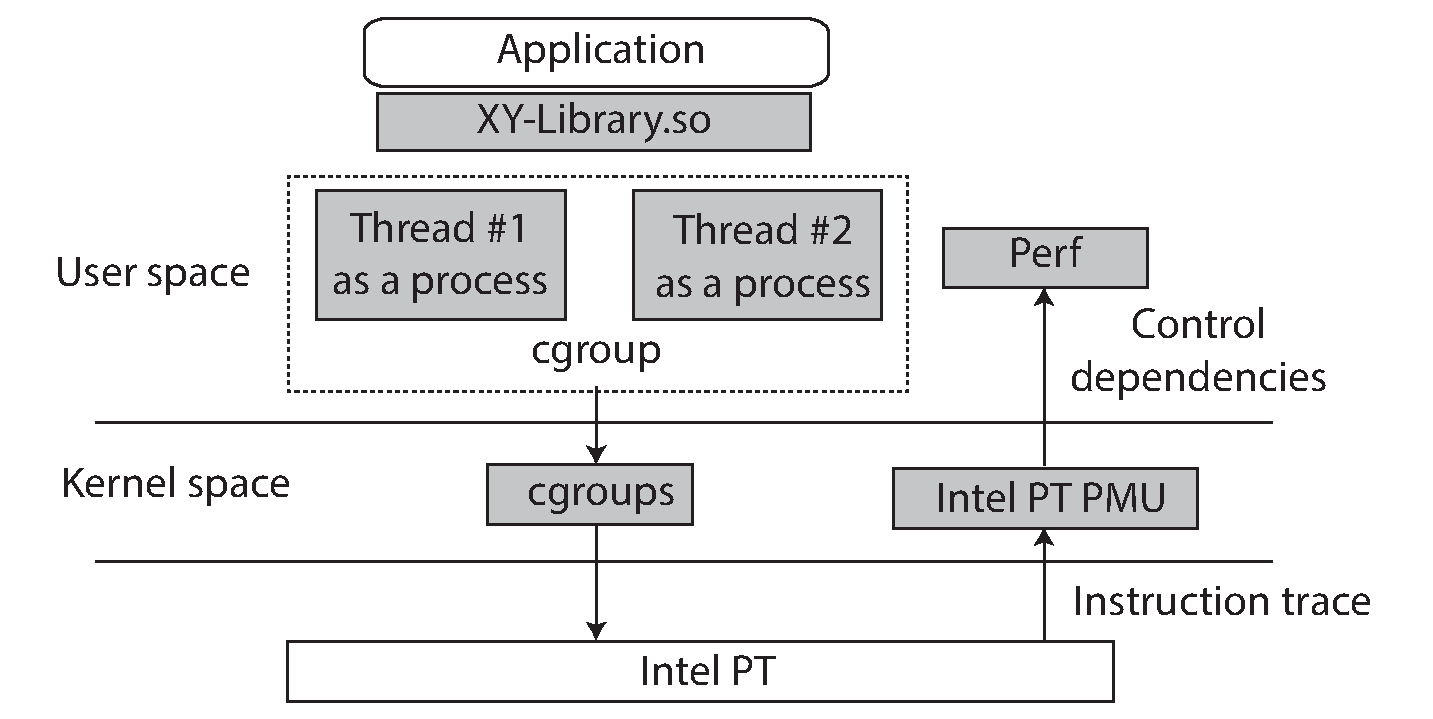
\includegraphics[scale=.35]{figure/PT-os}
  \caption{\projecttitle OS support.}
   
  \label{fig:pt-OS-support}

\end{figure}

%%\begin{figure}[h]
%%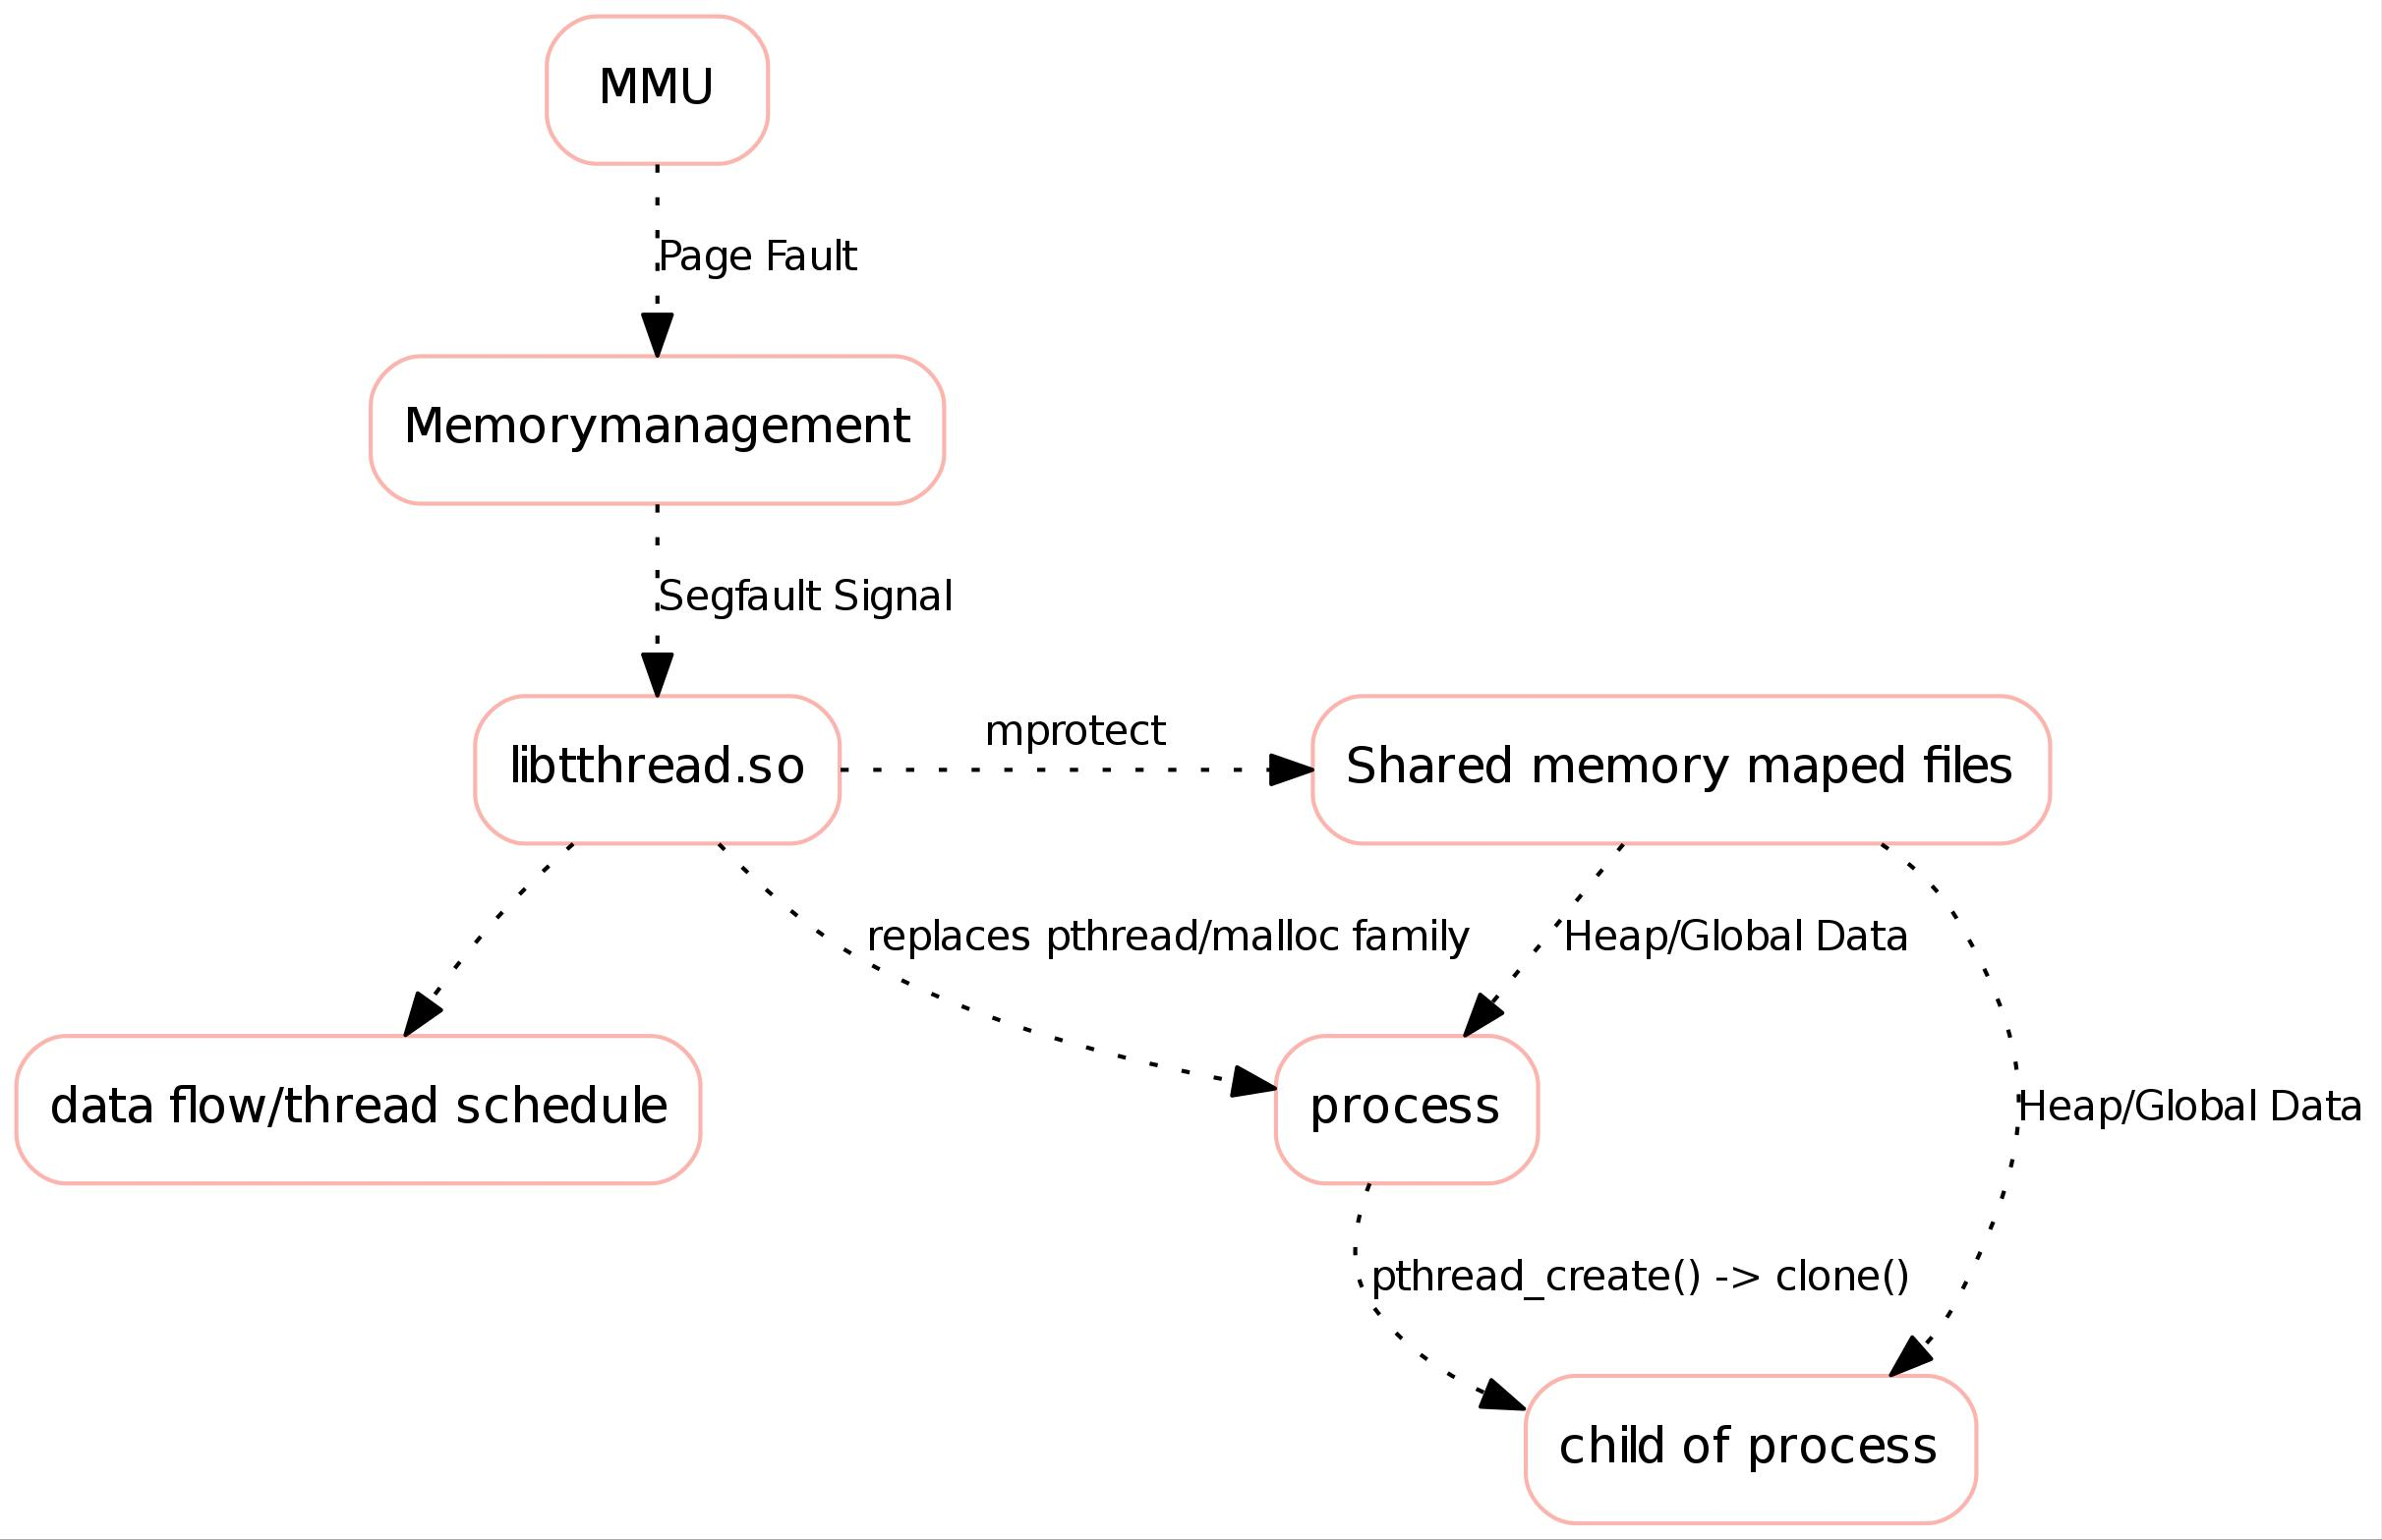
\includegraphics[width=8cm]{figure/arch.jpg}
%%\caption{Libtthread Architecture}
%%\label{fig:tthread}
%%\end{figure}
%%
%%\begin{figure}[h]
%%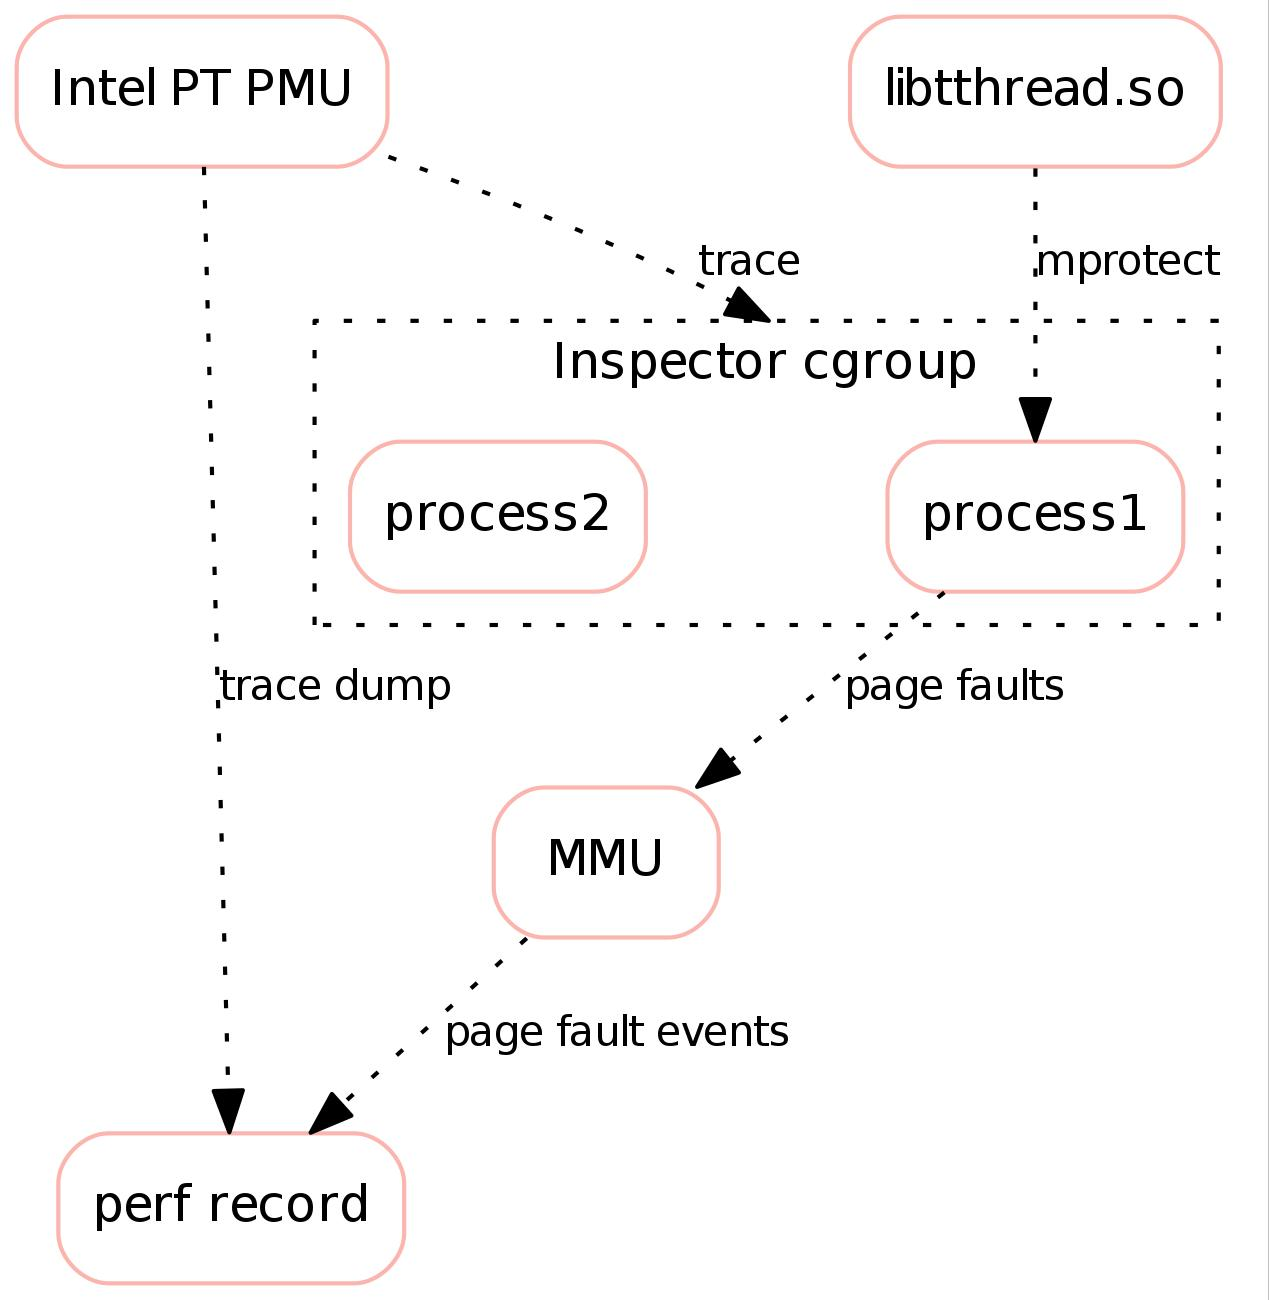
\includegraphics[width=8cm]{figure/arch2.jpg}
%%\caption{Inspector Architecture}
%%\label{fig:inspector}
%%\end{figure}
%
%Along with PT page fault events generated by the kernel will be included
%addionally to the trace packets. Because \emph{tthread} uses \emph{mprotect}
%syscall to monitor access of heap and global memory space, whenever the
%application access this memory, the MMU will generate page fault. These
%page fault also includes the location, where in code memory was accessed.
%
%After execution the result can be further processed by using a set of tools
%for example \emph{perf script}. The branch information is still in a compressed
%form and needs to be decoded. Perf has a decoder integrated to achieve this.
%To map the trace onto binaries, it needs access to executables and linked
%libraries of the application. During the excecution mmap events are tracked to
%know to the location of each loadable.

